Since the noise in GW detectors is very high, especially compared to the GW background, it makes sense to use powerful methods to separate the signal from the noise. One promising method is information field theory (IFT).
Information field theory is a technique for signal reconstruction
and field inference designed by Torsten Enßlin and his group at the 
Max Planck Institute in Garching.  Its goal is to use a formalism from Bayesian statistics and quantum field theory to be able to reuse methods to infer fields from data. The problem
at the base is that we want to infer a spatially continuously distributed field
from a finite amount of data. To do that, we can add our knowledge about 
physical laws, statistics, etc. of the problem, in the form of correlation functions.

We need to define our probability density functions over the space of all
possibilities, which is why we will integrate using path integrals in 
this formalism.

If we assume a linear measurement, our data consists of the signal modified by a response function and added noise. 

\begin{equation}
    d = R s + n
\end{equation}

It is reasonable to assume a linear response from our detector, see e.g. \cite{todo satyaprakash}. They derive an expression for the return time of the laser signal in the interferometer derived by time. This is proportional to the time derivative of the strain, here in plus polarisation. 

\begin{equation}
    \frac{dt_{return}}{dt}=1+\sin^2(\theta)L \dot{h}_+(t)
\end{equation}

Here, $\theta$ is the angle between the beam direction and the detector plane.

\begin{equation}
    (R s)_i = \int dx R_{ix} s_{x}
\end{equation}
The response corresponds to the point spread function of our instrument and
other linear operations performed on the data.

With Gaussian noise, we get the following likelihood:
\begin{equation}
    P(d|s) = \mathcal{N}(d-Rs, N) .
\end{equation}

\section{Information Hamiltonian}

Using Bayes theorem, we define what is called an information Hamiltonian.
\begin{equation}
    P(s|d) = \frac{P(d|s)P(s)}{P(d)}
\end{equation}
    
\begin{equation}
    = \frac{e^{-\mathcal{H}(d, s)}}{Z_d}
\end{equation}

Here, $Z_d$ is the partition function, which is the evidence here.
\begin{equation}
    Z_d = P(d)
\end{equation}
\begin{equation}
        \mathcal{H}(d, s) = -ln(P(d|s)) - ln(P(s))
\end{equation}

\section{Wiener Filter}
For a Gaussian prior and a Gaussian signal, we obtain the following
Hamiltonian.
\begin{equation}
    \mathcal{H}(d, s) = \frac{1}{2}(d-Rs)^{\dagger}N^{-1}(d-Rs)+\frac{1}{2}s^{\dagger}S^{-1}s
\end{equation}

With quadratic completion, we can rewrite this in canonical form.
\begin{equation}
    \mathcal{H}(d, s) = \frac{1}{2}(s-m)^\dagger D^{-1}(s-m)
\end{equation}
When applying the covariance to the source, we get the mean according to the Wiener filter.
\begin{equation}
    m = Dj
\end{equation}
\begin{equation}
    D =(S^{-1}+R^{\dagger}N^{-1}R)^{-1}
\end{equation}
\begin{equation}
    j =R^{\dagger}N^{-1}d
\end{equation}
The covariance can also be written with the signal and the mean:
\begin{equation}
    D=\langle (s-m)(s-m)^\dagger \rangle_{s|d}
\end{equation}
Here, we assume the detector response $R$, the noise covariance $N$ of the detector and the signal covariance $S$ coming from physical laws, here coming from the calculated angular power spectrum.

The posterior of the Wiener filter is a Gaussian distribution with mean $s-m$ and the earlier-mentioned covariance.
\begin{equation}
    P(s|d)=\mathcal{N}(s-m, D)
\end{equation}


\section{1D Toy Model}

To show how {\tt NIFTy} works in principle, we will reconstruct a one-dimensional power spectrum. From this input, a random realisation of data points is drawn from which the signal is reconstructed. The reconstruction and the residual plot are shown in Fig. \ref{1D_reconstruction}.In this case, the reconstruction works quite well. 

\begin{figure}[h]
    \centering
    \subfloat{
        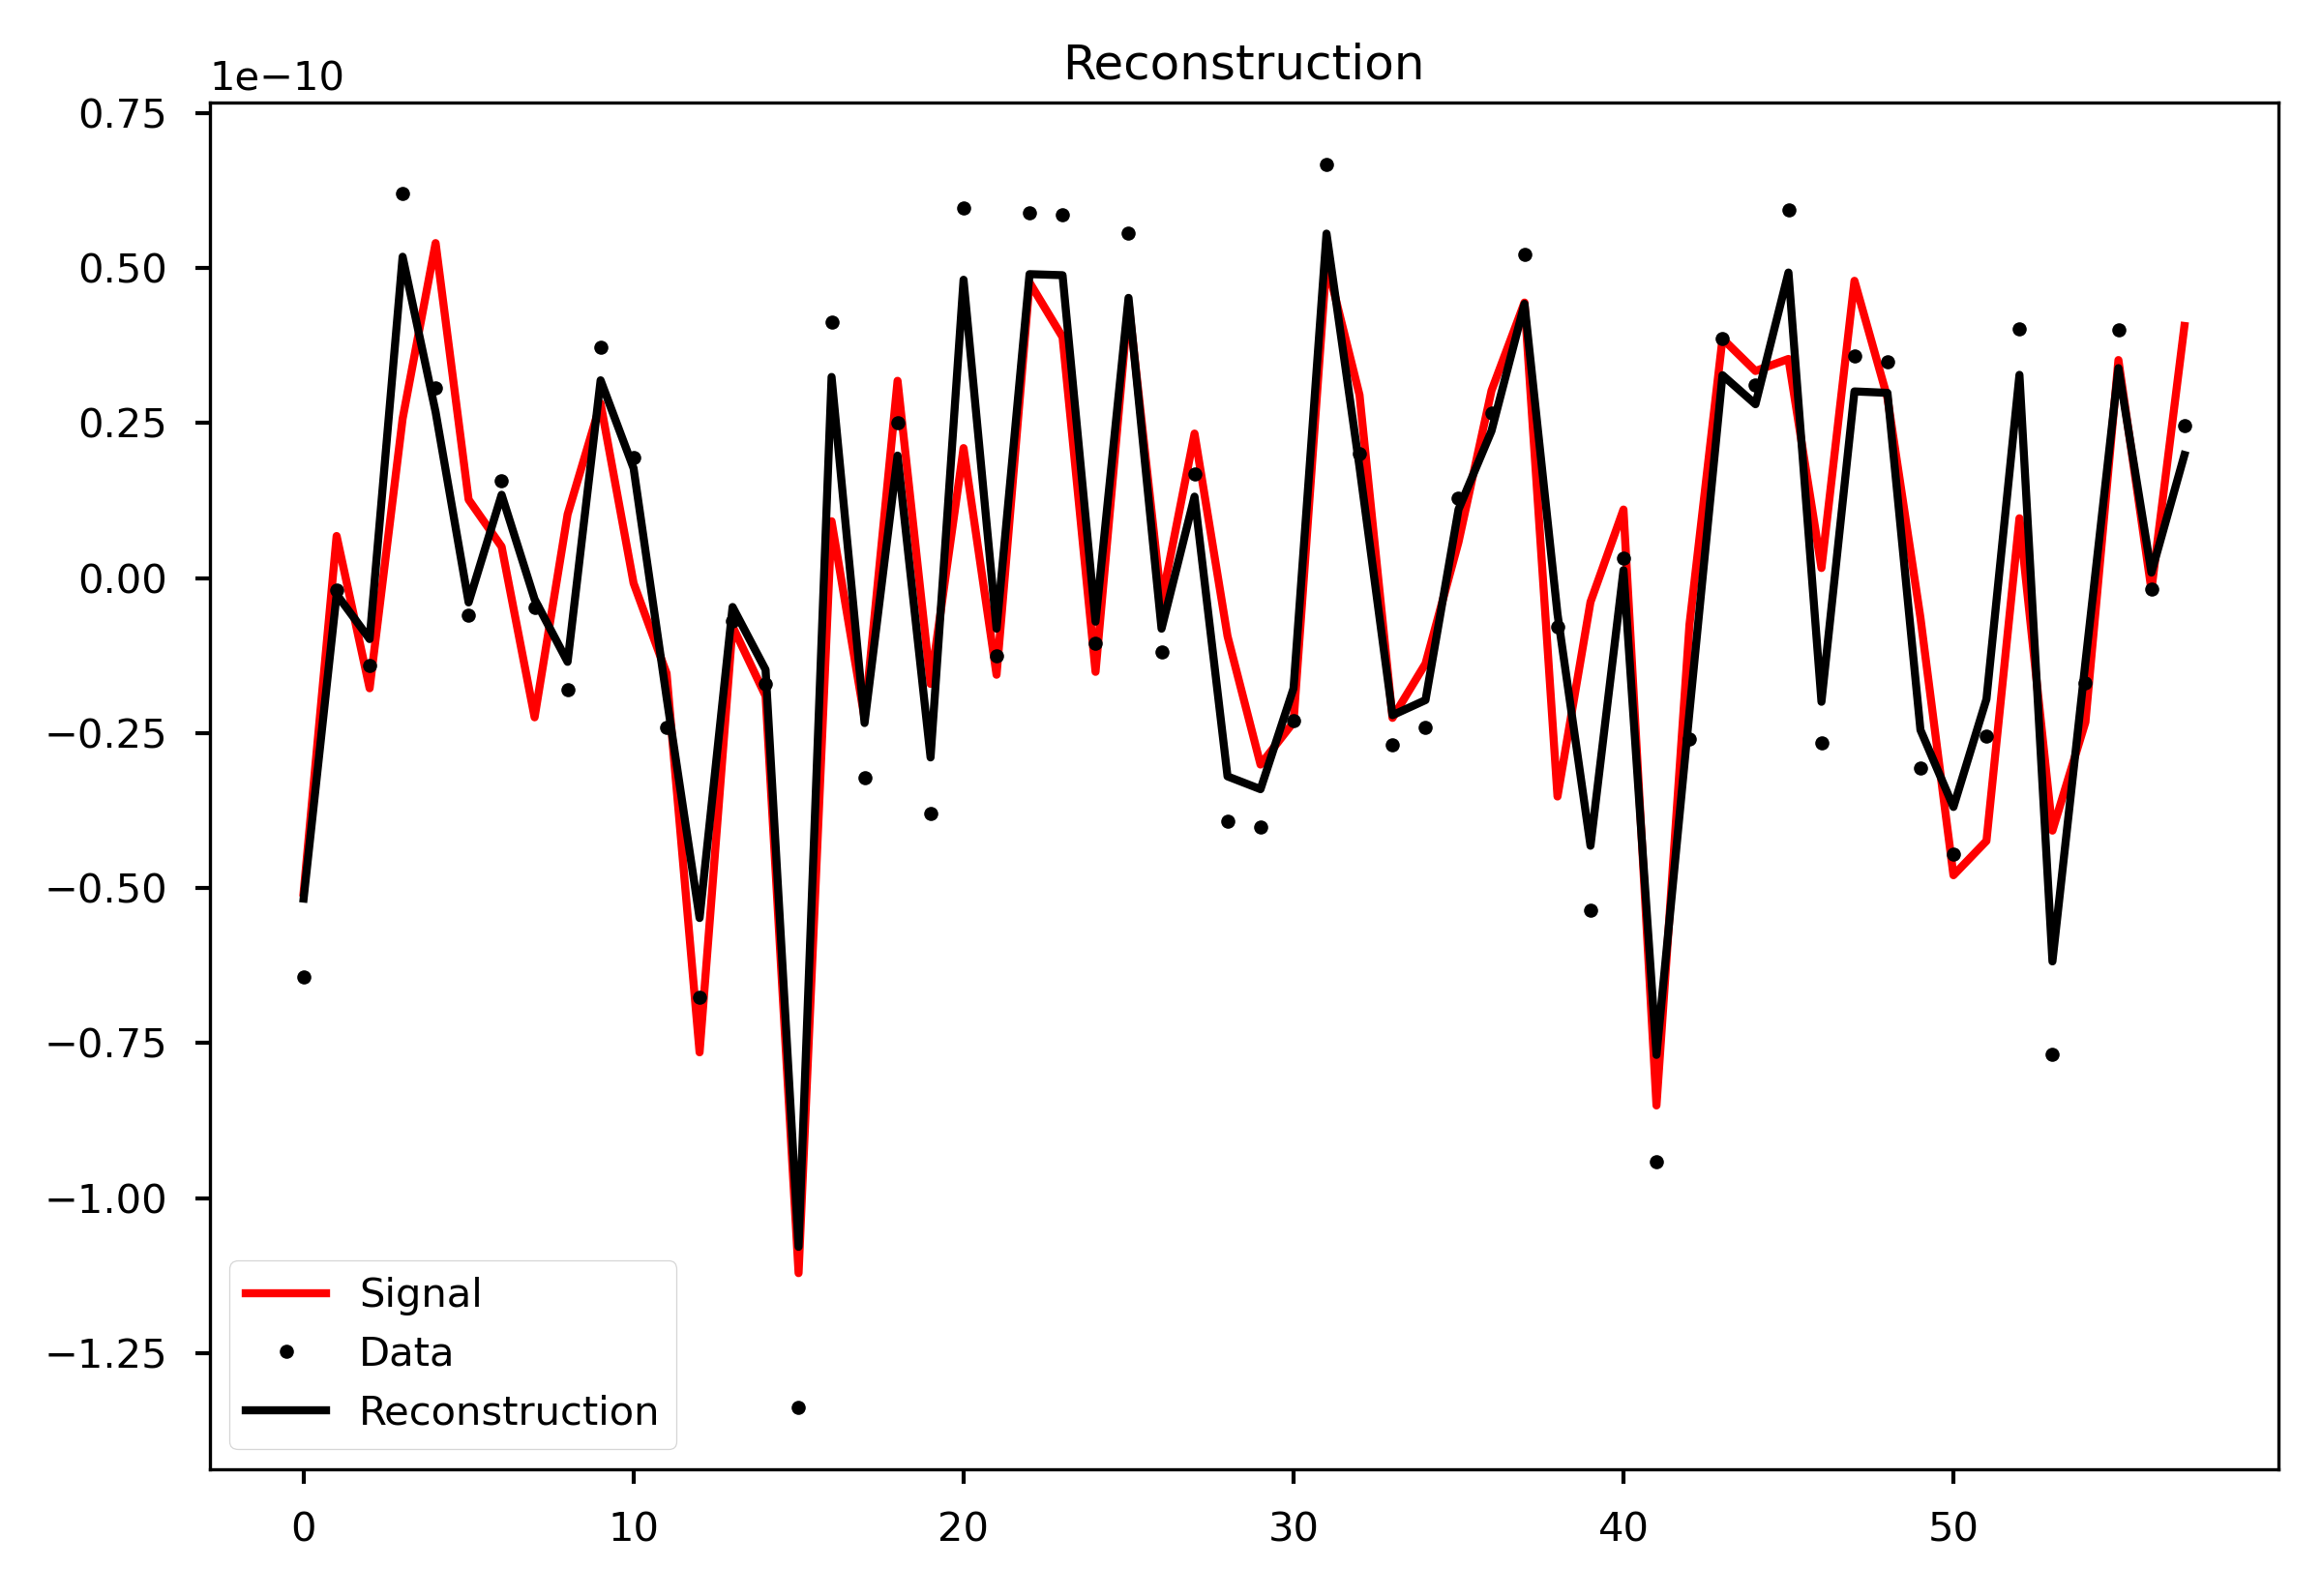
\includegraphics[width=7.5cm, clip]{Images/recon_400Hz_1D.png}}
    \subfloat{
        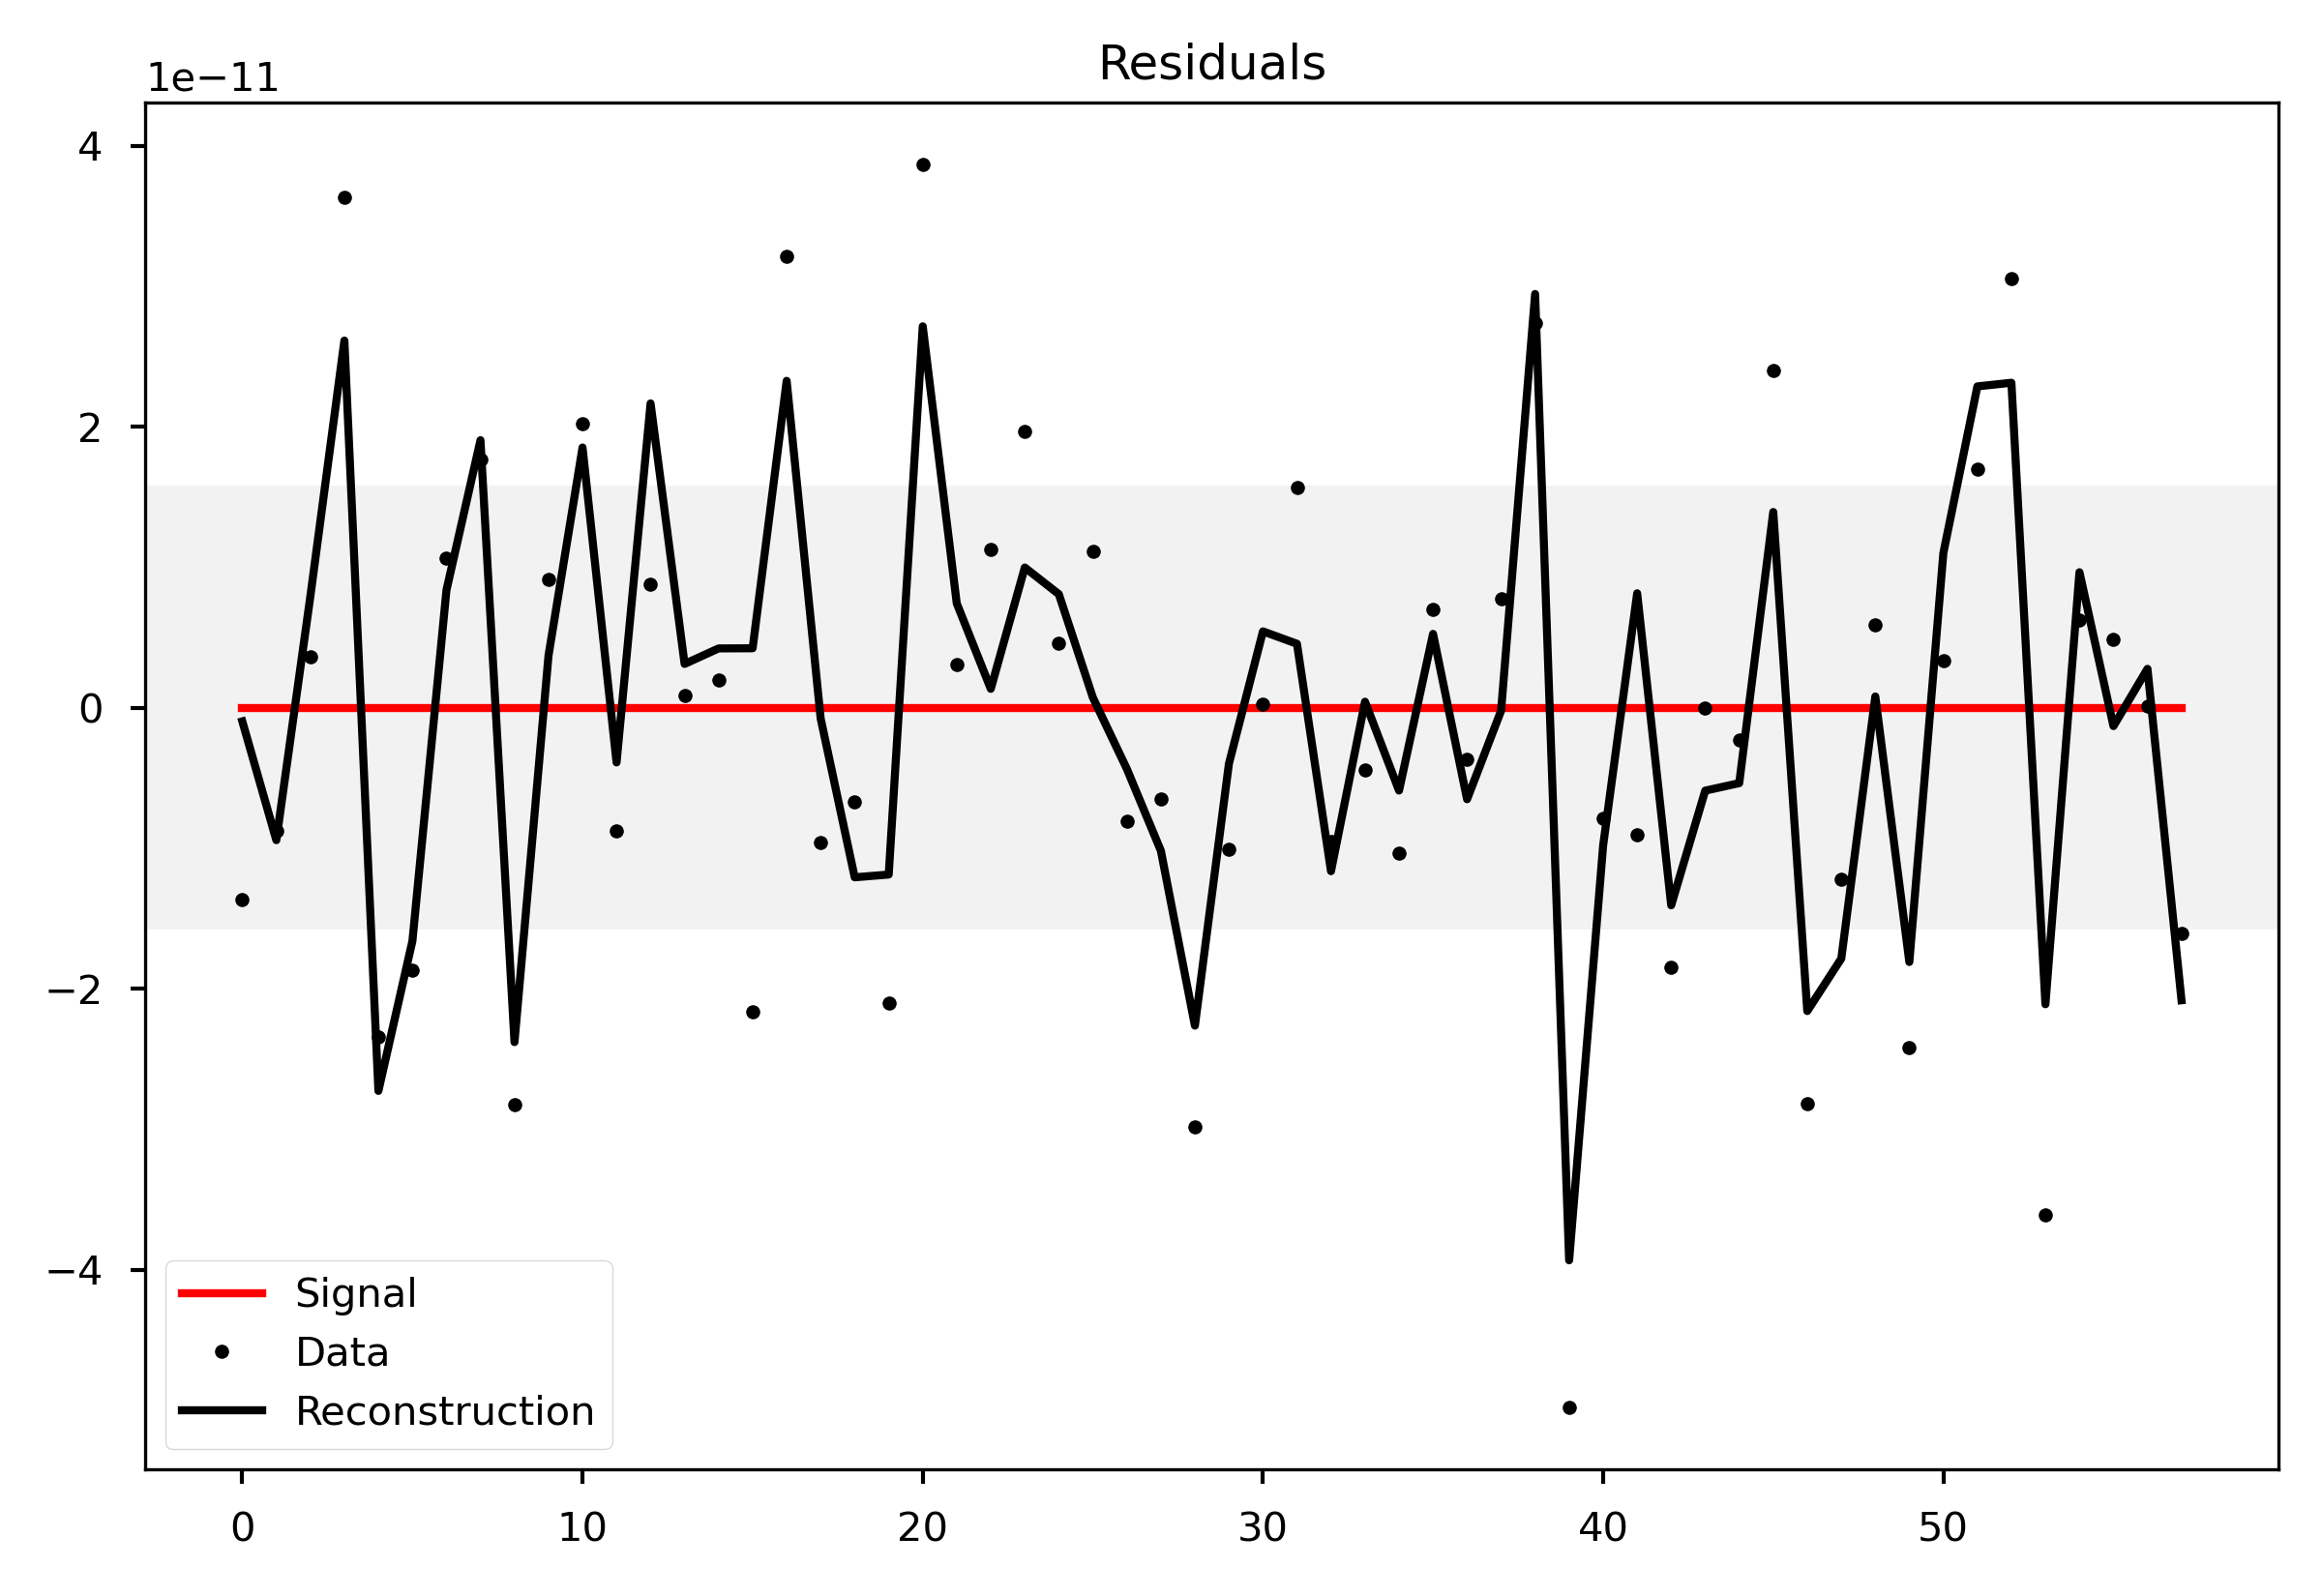
\includegraphics[width=7.5cm, clip]{Images/residuals_400Hz_1D.png}}
    \caption{An example of using the {\tt NIFTy} code to reconstruct an input power spectrum.}
    \label{1D_reconstruction}
\end{figure}

\begin{figure}[h]
    \centering
    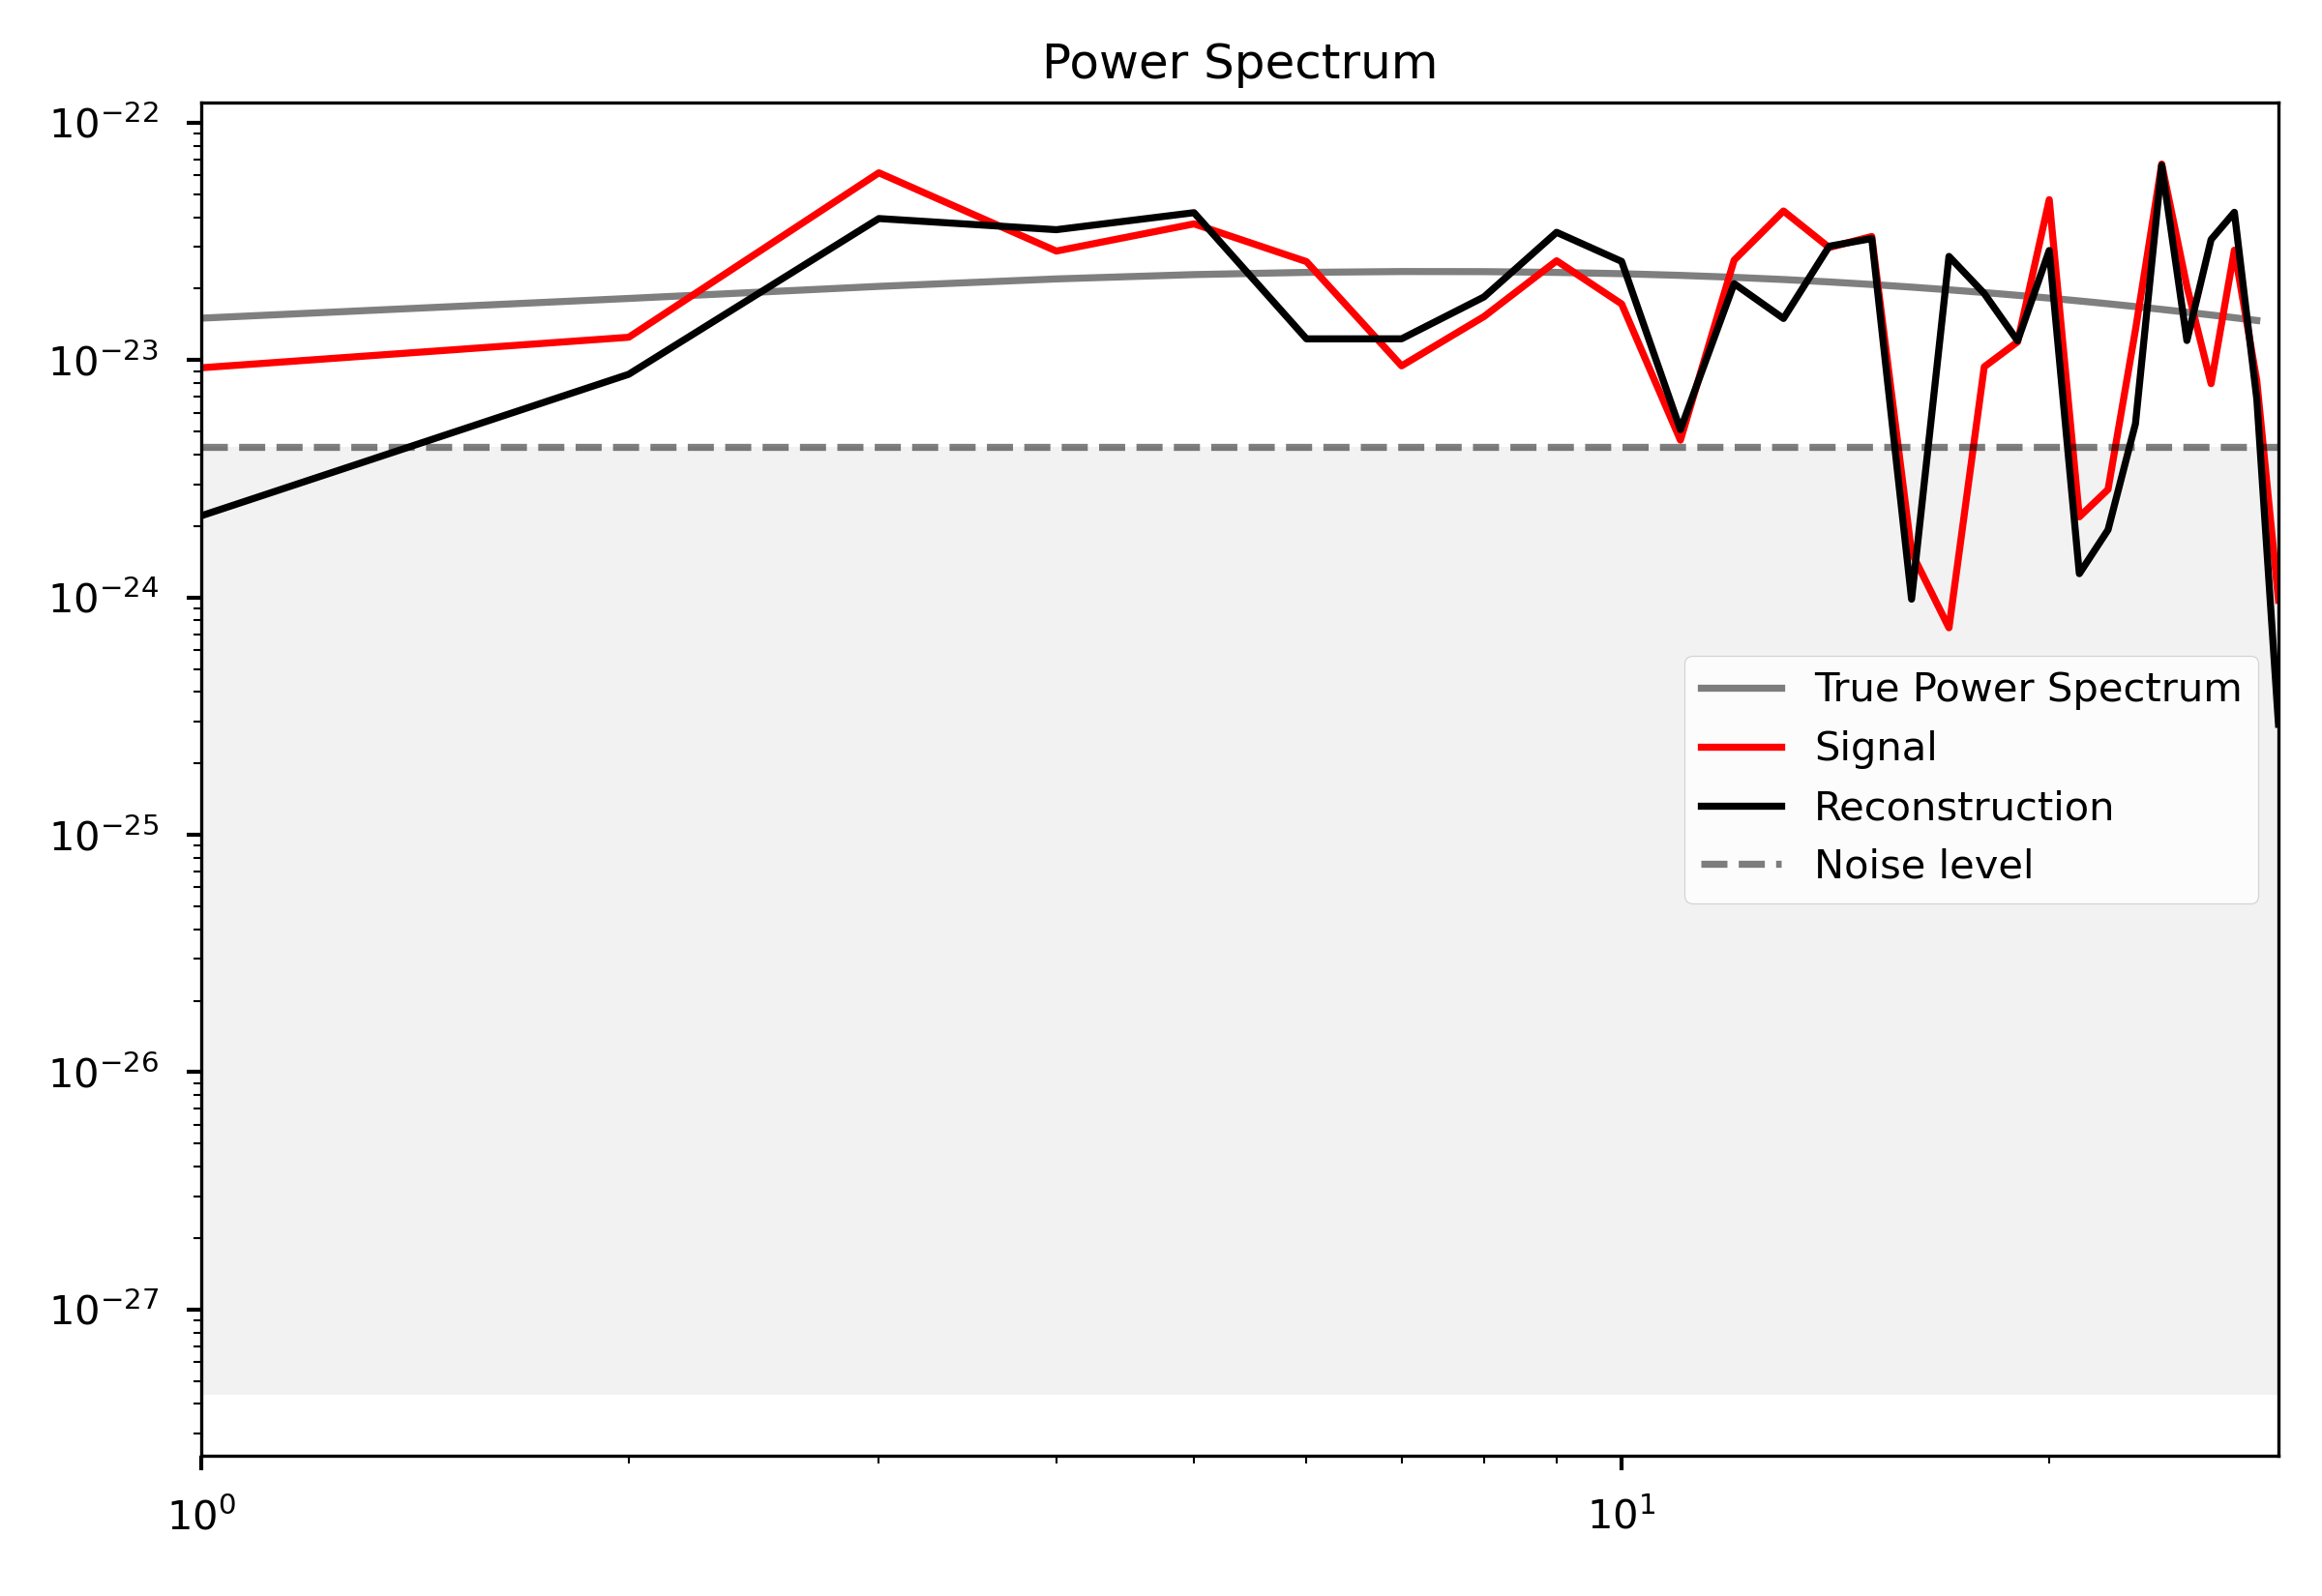
\includegraphics[width=0.7\linewidth]{Images/power_spectrum_400Hz_1D.png}
    \caption[The power spectra of the one-dimensional toy model.]{The power spectra of the one-dimensional toy model. The input power spectrum is shown in grey, the signal realisation in red and the reconstruction using IFT in black.}
    \label{1D_power_spectrum}
\end{figure} 

In Fig.\ref{1D_power_spectrum}, we show different power spectra, i.e. the input, the one from the randomly drawn signal and the reconstruction. The reconstruction power spectrum is very similar to the signal one in this toy model.
